%%%%%%%%%%%%%%%%%%%%%%%%%%%%%%%%%%%%%%% プリアンブル %%%%%%%%%%%%%%%%%%%%%%%%%%%%%%%%%%%%%%%
\documentclass[a4j,12pt]{jreport}
\usepackage{amsmath,amsthm,amssymb}
\usepackage{mathtools}
\usepackage[dvips]{color}
\usepackage[dvipdfmx]{graphicx}
\usepackage{enumerate}
\usepackage{algorithmic}
\usepackage{float}
\usepackage{subcaption}
\usepackage{longtable}
\usepackage{listings, jvlisting}
\usepackage{here}
\usepackage{bm}


%*** 定理等の環境設定 ***
\newtheoremstyle{theo}%name
  {5pt} % space above
  {5pt} % space below
  {\rm}  % bofy font
  {} % ident - empty=no indent,  \parindent= paragraph indent
  {\bf}  % thm head font
  { }    % punctuation after thm head
  { }    % space after thm head: `` ``=normal \newline=linebreak
  {}     % thm head specification
\theoremstyle{theo}
\newtheorem{theo}{定理}[chapter]
\newtheorem{lem}[theo]{補題}
\newtheorem{prop}[theo]{命題}
\newtheorem{coro}[theo]{系}
\newtheorem{defi}{定義}[chapter]
\newtheorem{ex}{例}[chapter]
\newtheorem{rem}{注意}
\renewcommand{\therem}{}
\renewcommand{\proofname}{\bfseries 証明}
\renewcommand{\qedsymbol}{$\square$}


%*** ページ内レイアウト ***
\topmargin -15mm
\textheight 250mm
\textwidth 165mm
\oddsidemargin -2.5mm

\newcommand{\ColorW}[1]{{\color{white}#1}}
%%%%%%%%%%%%%%%%%%%%%%%%%%%%%%%%%%%%%%%%%%%%%%%%%%%%%%%%%%%%%%%%%%%%%%%%%%%%%%%%%%%%%%%%





%%%%%%%%%%%%%%%%%%%%%%%%%%%%%%%%%%%%%%%%% 本文 %%%%%%%%%%%%%%%%%%%%%%%%%%%%%%%%%%%%%%%%%
\begin{document}

%#######################################################################################
%*** 表紙 ***
% 自分の「タイトル」，「学生番号」，「氏名」を入力してください．
%
\title{\LARGE 20xx年度　数学講究研究報告\\\vspace{1.5cm}
タイトル\\ % <- タイトル
{\huge　\\} \vspace{7cm}}
\author{
 \LARGE
 \centering
  \begin{tabular}{ll}
   学籍番号：200440000 \\  % <-- 学籍番号
   氏　　名：名城 太郎  % <-- 氏名 
  \end{tabular}
} 

\date{\vspace{1.5cm} \Large 名城大学　理工学部　数学科}
\pagestyle{empty}
\maketitle
%#######################################################################################





%#######################################################################################
%*** 目次 ***
% この部分は変更しないでください．
%
\pagenumbering{roman}  % 目次のページ番号を"roman"で出力
\tableofcontents % 目次作成
\cleardoublepage
\pagestyle{plain}
\pagenumbering{arabic} % 目次のページ番号を"arabic"で出力
\baselineskip 4ex
%#######################################################################################





%#######################################################################################
\chapter*{要約} \addcontentsline{toc}{chapter}{要約}
%#######################################################################################

研究報告の内容を1ページ程度で要約したもの．
作成した研究報告には何が書かれているかを読む人に伝える必要があります．
学会誌などに投稿する論文でも書きます．
 読む人はここに書かれていることを参考にして，その論文を読むか読まないかを判断することが多いです．







\newpage
%#######################################################################################
\chapter{はじめに}
%#######################################################################################
数学講究では，1年間に学んだ内容を数学講究研究報告（他学科の卒業論文に相当するもの）としてまとめます．
基本的に数学講究研究報告は，LATEXで書きます．
LATEXでは，数式を書くための様々なコマンドが用意されており，理工学系の文書作成のために広く利用されています．
提出時期は1月末頃で，指導教員に提出します．

このファイルの内容を参考にして，数学講究研究報告を作成してください．
基本的には，このファイルの不要な部分を削除し，自分の内容を入力していけばよいです．
また，作成前に別ファイルの「数学講究について」を熟読してください．

\bigskip
なお，数学講究研究報告の「はじめに」では，研究の背景・目的を書き，この研究報告でどのようなことを示すのかを簡潔の述べます．
数学講究でどのようなテキストを使い何について学んだのか．
また，その中で自分は何に興味を持ちどのような内容についてまとめるのか．
この研究報告が章ごとにどのような構成になっているのかなどを簡潔に書いてください．





\newpage
%#######################################################################################
\chapter{準備}
%#######################################################################################
%&&&&&&&&&&&&&&&&&&&&&&&&&&&&&&&&&&&&&&&&&&&&&&&&&&&&&&&&&&&&&&&&&&&&&&&&&
\section{準備について}
%&&&&&&&&&&&&&&&&&&&&&&&&&&&&&&&&&&&&&&&&&&&&&&&&&&&&&&&&&&&&&&&&&&&&&&&&&
次章の本論で必要となる定義や定理についてまとめる．
 また，次章ではそれらを適切に参照して説明していく．
長くなる場合は，2.1，2.2，$\ldots$のように，内容ごとに節に分けてもよい．



%&&&&&&&&&&&&&&&&&&&&&&&&&&&&&&&&&&&&&&&&&&&&&&&&&&&&&&&&&&&&&&&&&&&&&&&&&
\section{LATEXの使い方の例}
%&&&&&&&&&&&&&&&&&&&&&&&&&&&&&&&&&&&&&&&&&&&&&&&&&&&&&&&&&&&&&&&&&&&&&&&&&
実際に，数学講究研究報告を書くときの参考のためLATEXの使い方について以下で簡単に説明する．



%+++++++++++++++++++++++++++++++++++++++++++++++++++++++++++++++++++++++++++++++++++++++
\subsection*{定義等の環境} % <- 長くなる場合は，内容ごとに「\subsection*」で適切に分割してください．
%+++++++++++++++++++++++++++++++++++++++++++++++++++++++++++++++++++++++++++++++++++++++
定義等については，あらかじめそれぞれの環境が用意されているので，それを利用してください．
使い方については，以下を参考にしてください．
%=======================================================================================
\begin{defi} % *** 定義 ***
定義の内容を書く．
\end{defi}
%=======================================================================================
%=======================================================================================
\begin{theo} \label{theo:2.1}%*** 定理 ***
定理の内容を書く．
\end{theo}
%***********
\begin{rem}
定理等について補足することがあれば，注意として書いておくとよい．
\end{rem}
%***********
\begin{proof}
ここに証明を書く．
\end{proof}
%=======================================================================================
%=======================================================================================
\begin{lem} \label{lem:2.2}%*** 補題 ***
補題の内容を書く．
\end{lem}
%***********
\begin{proof}
ここに証明を書く．
\end{proof}
%=======================================================================================
%=======================================================================================
\begin{prop} %*** 命題 ***
命題の内容を書く．
\end{prop}
%***********
\begin{proof}
ここに証明を書く．\\
補題\ref{lem:2.2}から，次が成り立つ． % <- labelをつけて参照することができる．
\end{proof}
%=======================================================================================
%=======================================================================================
\begin{coro} %*** 系 ***
系の内容を書く．
\end{coro}
%***********
\begin{proof}
ここに証明を書く．
\end{proof}
%=======================================================================================
%=======================================================================================
\begin{ex} %*** 例 ***
例を書く．
\end{ex}
%=======================================================================================
「定理」，「命題」，「補題」，「系」は，定義などから導出される数学的主張について述べる際に使います．
著者により，多少使い方が異なることもありますが，だいたい次のように使い分けるとよいです．
\begin{itemize}
 \item \textbf{定理}：論文中で特に強調して主張したいこと．
 \item \textbf{命題}：強調するほどでもないが，ある程度重要で主張したいこと．
 \item \textbf{補題}：定理，命題を証明するために必要な数学的主張．
 \item \textbf{系}：定理・命題から得られる比較的容易に証明できる主張．
                        定理・命題の帰結として用いるとよい．
\end{itemize}
上記については，厳密なルールはないので，読む人が内容を理解しやすいように使い分けられていればそれでよいです．
また，テキストで「定理」と書いてあるからといって，同様に「定理」とする必要はありません．
自分の研究報告の内容に合わせて使い分けてください．



%+++++++++++++++++++++++++++++++++++++++++++++++++++++++++++++++++++++++++++++++++++++++
\subsection*{数式環境} 
%+++++++++++++++++++++++++++++++++++++++++++++++++++++++++++++++++++++++++++++++++++++++
\begin{itemize}
 \item 文章中で数式を使う場合は，「\$数式\$」とします．
 例えば，$y = ax^2 + bx + c$です．
 \item 1行の数式を中央に書きたい場合は
         $$
           y = ax^2 + bx + c
         $$
         または
         \[
           y = ax^2 + bx + c
         \]
         とします．
 \item 複数行の数式を書くための環境はいくつかありますが，以下の環境を使ってください．
         \begin{align} \label{eq:2.1}
           (x - 2y)(x - 2y + 5) + 6 &= (x - 2y) \{(x - 2y) + 5\} + 6 \nonumber\\
            &= (x - 2y)^2 + 5(x - 2y) + 6 \nonumber\\
            &= \{ (x - 2y) + 2 \} \{ (x - 2y) + 3 \} \nonumber\\
            &= (x - 2y + 2 )( x - 2y + 3 ) 
         \end{align}
         「\&」の位置で，各行の開始位置が決まります．
         ラベルをつけて，式(\ref{eq:2.1})のように参照することもできます．
         「\verb|\nonumber|」がないと式番号が表示されます．
         式番号は参照するもの以外にはつけないほうがよいです．
 \item 式番号なしで複数行の数式を書く場合は，以下の環境を使ってください．
         \begin{align*} 
           (x - 2y)(x - 2y + 5) + 6 &= (x - 2y) \{(x - 2y) + 5\} + 6 \\
            &= (x - 2y)^2 + 5(x - 2y) + 6 \\
            &= \{ (x - 2y) + 2 \} \{ (x - 2y) + 3 \} \\
            &= (x - 2y + 2 )( x - 2y + 3 ) 
         \end{align*}
         上記の環境を使うと， 「\verb|\nonumber|」を書かなくてよくなります．
\end{itemize}



%+++++++++++++++++++++++++++++++++++++++++++++++++++++++++++++++++++++++++++++++++++++++
\subsection*{よく使う数学記号} 
%+++++++++++++++++++++++++++++++++++++++++++++++++++++++++++++++++++++++++++++++++++++++
\begin{itemize}
  \item $x^2$，$(a_k)^5$
  \item $\alpha$，$\beta$，$\gamma$，$\omega$，$\pi$，$\lambda$，$\epsilon$，$\varepsilon$，$\delta$，$\mu$，$\sigma$，$\Gamma$，$\Omega$，$\Pi$
  \item $\mathcal{A}$，$\mathcal{B}$，$\mathcal{F}$，$\mathbb{R}$，$\mathbb{C}$，$\mathbb{N}$，$\mathbb{Z}$，
          $\mathrm{P}$，$\mathrm{Pr}$，$\mathrm{E}$，$\mathrm{V}$，$\mathrm{Var}$  
  \item $\sin x$，$\cos x$，$\tan x$，$\log x$，$e^x$，$\exp[x]$
  \item $k=1, 2, \ldots, n$，$a_1 + a_2 + \cdots + a_n$
  \item $\le$，$\ge$，$\leqq$，$\geqq$，$<$，$>$，$=$，$\ne$，$\pm$，$\mp$
  \item $\Leftarrow$，$\Rightarrow$，$\Leftrightarrow$，$\Longleftrightarrow$，$\lim_{n \to \infty}$
  \item $x \in A$，$x \notin \mathbb{R}$，$A \subset B$，$A \cap B$，$A \cup B$，
          $\bigcap_{k=1}^{\infty}A_n$，$\bigcup_{k=1}^{\infty}A_n$，$A^c$，$\bar{A}$，$\overline{A}$，$\emptyset$
  \item ${}_n \mathrm{C}_k$，$\binom{n}{k}$，$n!$
  \item $ \sum_{k=1}^{\infty} a_k$，$\prod_{k=1}^{n}a_k$
  \item $f^{\prime}(x)$，$f^{\prime \prime}(x)$，$\frac{dy}{dx}$，$\int \sin x \;dx$，$\int_{a}^{b} (2x^3 - 3x + 5 ) \;dx$
  \item $\frac{1}{2}$，$x^{\frac{1}{n}}$，$\sqrt{2}$，$\sqrt[n]{5}$
  \item $
           |a|=
           \begin{cases}
             a, & a \geqq 0, \\
             -a, & a < 0.
           \end{cases}
          $
  \item $
            A =
            \begin{pmatrix}
              1 & 2 & 3 \\
              4 & 5 & 6 \\
              7 & 8 & 9
            \end{pmatrix}
          $，
          $
            P =
            \begin{pmatrix}
              p_{1,1} & p_{1,2} & \cdots & p_{1,n} \\
              p_{2,1} & p_{2,2} & \cdots & p_{2,n} \\
              \vdots & \vdots & \ddots & \vdots \\
              p_{n,1} & p_{n,2} & \cdots & p_{n,n}\\
            \end{pmatrix}
          $，
          $
            |A| =
            \begin{vmatrix}
              1 & 2 & 3 \\
              4 & 5 & 6 \\
              7 & 8 & 9
            \end{vmatrix}
            =
            \left|
            \begin{matrix}
              1 & 2 & 3 \\
              4 & 5 & 6 \\
              7 & 8 & 9
            \end{matrix}
            \right|
          $
  \item $\left\{ \left( \frac{1}{2} \cdot \frac{3}{5} \right) \right\}$，$a\, b\; c\quad d\qquad$    
\end{itemize}



%+++++++++++++++++++++++++++++++++++++++++++++++++++++++++++++++++++++++++++++++++++++++
\subsection*{箇条書き} 
%+++++++++++++++++++++++++++++++++++++++++++++++++++++++++++++++++++++++++++++++++++++++
%*** 普通の箇条書き ***
\begin{itemize}
  \item 1つ目
          \begin{itemize}
            \item あいうえお
            \item アイウエオ
          \end{itemize} 
  \item 2つ目
          \begin{itemize}
            \item[$\Box$] 12345
            \item[$\Box$] abcde
          \end{itemize} 
  \item 3つ目
\end{itemize}

%*** 番号付き箇条書き ***
\begin{enumerate}[1.]
  \item 1つ目
          \begin{enumerate}[(1)]
            \item あいうえお
            \item アイウエオ
          \end{enumerate}
  \item 2つ目
          \begin{enumerate}[(i)]
            \item 12345
            \item abcde
          \end{enumerate}
  \item 3つ目
          \begin{enumerate}[(a)]
            \item 6789
            \item xyz
          \end{enumerate}
\end{enumerate}



\newpage
%+++++++++++++++++++++++++++++++++++++++++++++++++++++++++++++++++++++++++++++++++++++++
\subsection*{表の作成} 
%+++++++++++++++++++++++++++++++++++++++++++++++++++++++++++++++++++++++++++++++++++++++
LATEXでは，以下のように表を作成することができます．
思ったところに表を出力するのに苦労することもある．
\begin{table}[htbp]
  \centering
  \begin{tabular}{|c||c|c|c|} \hline
    $n$ & $n^2$ & $\sqrt{n}$ & $\frac{1}{n}$ \\ \hline\hline
     1 &  1 & 1.0000 & 1.0000 \\ 
     2 &  4 & 1.4142 & 0.5000 \\ 
     3 &  9 & 1.7321 & 0.3333 \\ 
     4 & 16 & 2.0000 & 0.2500 \\ 
     5 & 25 & 2.2361 & 0.2000 \\ \hline
     6 & 36 & 2.4495 & 0.1667 \\ 
     7 & 49 & 2.6458 & 0.1429 \\ 
     8 & 64 & 2.8284 & 0.1250 \\ 
     9 & 81 & 3.0000 & 0.1111 \\ 
    10 & 100 & 3.1623 & 0.1000 \\ \hline
  \end{tabular}
\end{table}



\newpage
%+++++++++++++++++++++++++++++++++++++++++++++++++++++++++++++++++++++++++++++++++++++++
\subsection*{図の作成と挿入} 
%+++++++++++++++++++++++++++++++++++++++++++++++++++++++++++++++++++++++++++++++++++++++
Microsoft OfficeのPowerPointで図を作成して，エクスポートでpdfファイルにすれば，以下のようにLATEXでも利用できます． 
\begin{figure}[htbp]
  \centering
  
\includegraphics[width=5cm]{図1.pdf}
  \caption{PowerPointで作成した図．}
\end{figure}

WinTpicというツールでLATEXに挿入できるグラフ・図を作成することができます．
このツールが無償で公開されています．
このツールで作成した図は，texファイルで保存できます．
例えば，次のような図が作成できます．
\begin{figure}[htbp]
  \centering
  %WinTpicVersion4.30d
{\unitlength 0.1in%
\begin{picture}( 16.1000, 18.1000)(  1.9000,-20.1000)%
% STR 2 0 3 0 Black White
% 4 990 1197 990 1210 4 190 0 0
% O
\put(9.9000,-12.1000){\makebox(0,0)[rt]{O}}%
% STR 2 0 3 0 Black White
% 4 960 187 960 200 4 190 0 0
% $y$
\put(9.6000,-2.0000){\makebox(0,0)[rt]{$y$}}%
% STR 2 0 3 0 Black White
% 4 1800 1227 1800 1240 4 190 0 0
% $x$
\put(18.0000,-12.4000){\makebox(0,0)[rt]{$x$}}%
% VECTOR 2 0 3 0 Black White
% 2 1000 2010 1000 200
% 
\special{pn 8}%
\special{pa 1000 2010}%
\special{pa 1000 200}%
\special{fp}%
\special{sh 1}%
\special{pa 1000 200}%
\special{pa 980 267}%
\special{pa 1000 253}%
\special{pa 1020 267}%
\special{pa 1000 200}%
\special{fp}%
% VECTOR 2 0 3 0 Black White
% 2 190 1200 1800 1200
% 
\special{pn 8}%
\special{pa 190 1200}%
\special{pa 1800 1200}%
\special{fp}%
\special{sh 1}%
\special{pa 1800 1200}%
\special{pa 1733 1180}%
\special{pa 1747 1200}%
\special{pa 1733 1220}%
\special{pa 1800 1200}%
\special{fp}%
% FUNC 2 0 3 0 Black White
% 10 190 200 1800 2010 1000 1200 1200 1200 1000 1000 192 200 1800 2010 0 2 0 0 1 0
% x^2
\special{pn 8}%
\special{pa 553 200}%
\special{pa 555 210}%
\special{pa 570 276}%
\special{pa 590 360}%
\special{pa 610 440}%
\special{pa 625 497}%
\special{pa 630 515}%
\special{pa 635 534}%
\special{pa 650 588}%
\special{pa 670 656}%
\special{pa 685 704}%
\special{pa 690 719}%
\special{pa 695 735}%
\special{pa 710 780}%
\special{pa 730 836}%
\special{pa 750 888}%
\special{pa 770 936}%
\special{pa 790 980}%
\special{pa 810 1020}%
\special{pa 830 1056}%
\special{pa 850 1088}%
\special{pa 870 1116}%
\special{pa 890 1140}%
\special{pa 910 1160}%
\special{pa 930 1176}%
\special{pa 950 1188}%
\special{pa 970 1196}%
\special{pa 990 1200}%
\special{pa 1010 1200}%
\special{pa 1030 1196}%
\special{pa 1050 1188}%
\special{pa 1070 1176}%
\special{pa 1090 1160}%
\special{pa 1110 1140}%
\special{pa 1130 1116}%
\special{pa 1150 1088}%
\special{pa 1170 1056}%
\special{pa 1190 1020}%
\special{pa 1210 980}%
\special{pa 1230 936}%
\special{pa 1250 888}%
\special{pa 1270 836}%
\special{pa 1290 780}%
\special{pa 1305 735}%
\special{pa 1310 719}%
\special{pa 1315 704}%
\special{pa 1330 656}%
\special{pa 1350 588}%
\special{pa 1365 534}%
\special{pa 1370 515}%
\special{pa 1375 497}%
\special{pa 1390 440}%
\special{pa 1410 360}%
\special{pa 1430 276}%
\special{pa 1445 210}%
\special{pa 1447 200}%
\special{fp}%
% FUNC 2 0 3 0 Black White
% 10 190 200 1800 2010 1000 1200 1200 1200 1000 1000 192 200 1800 2010 0 2 0 0 0 0
% x+2
\special{pn 8}%
\special{pa 190 1610}%
\special{pa 1600 200}%
\special{fp}%
% LINE 3 0 3 0 Black White
% 14 1300 740 1000 1040 1260 840 1000 1100 1220 940 1000 1160 1150 1070 1030 1190 1320 660 1000 980 1350 570 1000 920 1370 490 1000 860
% 
\special{pn 4}%
\special{pa 1300 740}%
\special{pa 1000 1040}%
\special{fp}%
\special{pa 1260 840}%
\special{pa 1000 1100}%
\special{fp}%
\special{pa 1220 940}%
\special{pa 1000 1160}%
\special{fp}%
\special{pa 1150 1070}%
\special{pa 1030 1190}%
\special{fp}%
\special{pa 1320 660}%
\special{pa 1000 980}%
\special{fp}%
\special{pa 1350 570}%
\special{pa 1000 920}%
\special{fp}%
\special{pa 1370 490}%
\special{pa 1000 860}%
\special{fp}%
% LINE 3 0 3 0 Black White
% 12 1000 920 840 1080 1000 980 870 1110 1000 1040 900 1140 1000 1100 930 1170 1000 1160 970 1190 1000 860 820 1040
% 
\special{pn 4}%
\special{pa 1000 920}%
\special{pa 840 1080}%
\special{fp}%
\special{pa 1000 980}%
\special{pa 870 1110}%
\special{fp}%
\special{pa 1000 1040}%
\special{pa 900 1140}%
\special{fp}%
\special{pa 1000 1100}%
\special{pa 930 1170}%
\special{fp}%
\special{pa 1000 1160}%
\special{pa 970 1190}%
\special{fp}%
\special{pa 1000 860}%
\special{pa 820 1040}%
\special{fp}%
\end{picture}}%

  \caption{WinTpicで作成した図．}
\end{figure}

また，Scilabという数値計算ソフトが無償で公開されています．
このソフトを使えば数値計算を行った結果をグラフで出力することができ，その図をLATEXで利用することができます．
\begin{figure}[htbp]
  \centering
  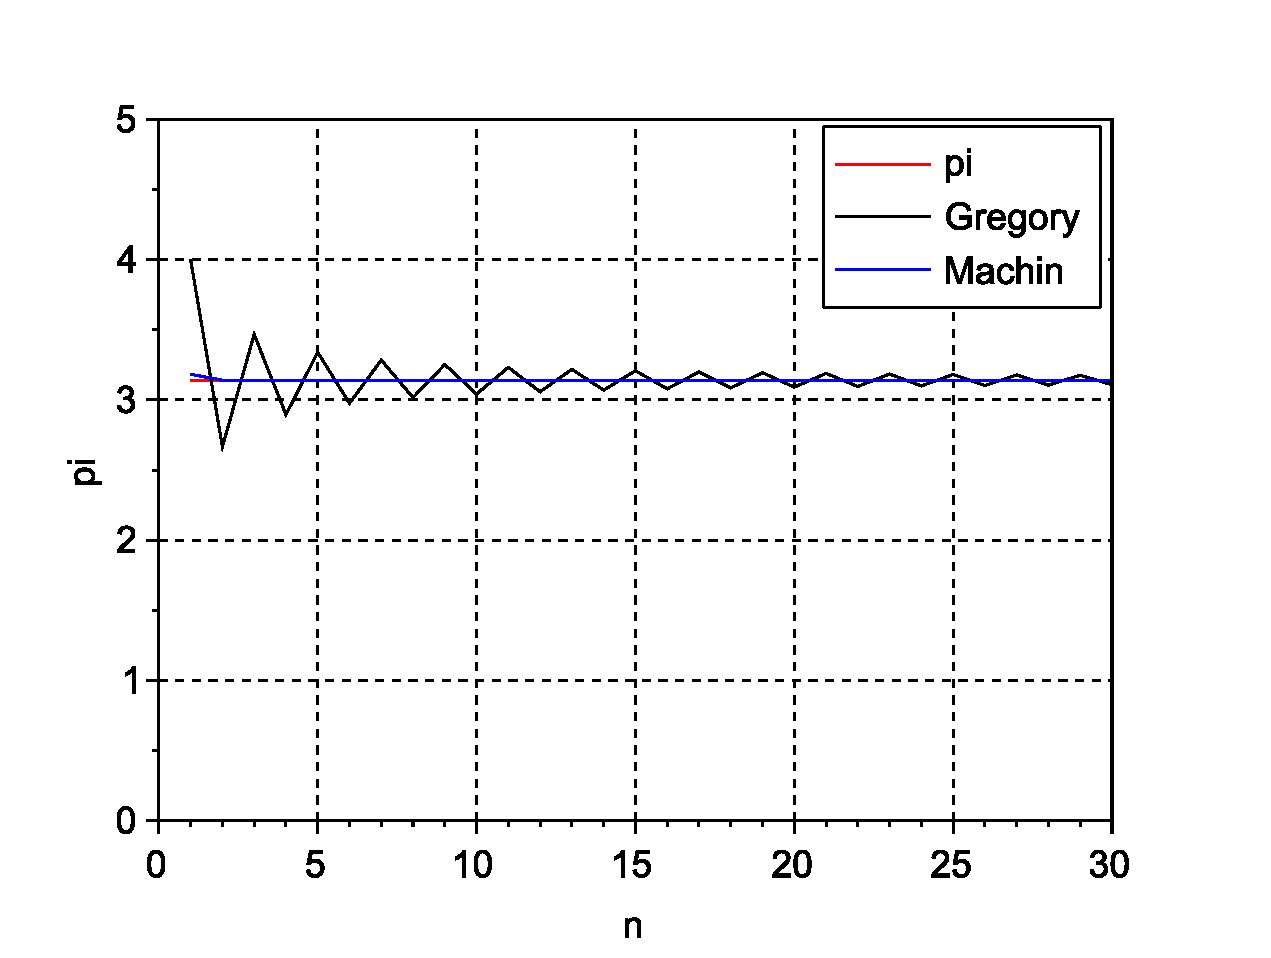
\includegraphics[width=7cm]{図3.pdf}
  \caption{Scilabで作成した図．}
\end{figure}


\begin{figure}[htbp]
   \centering
   \begin{tabular}{|c|c|}
    \hline
    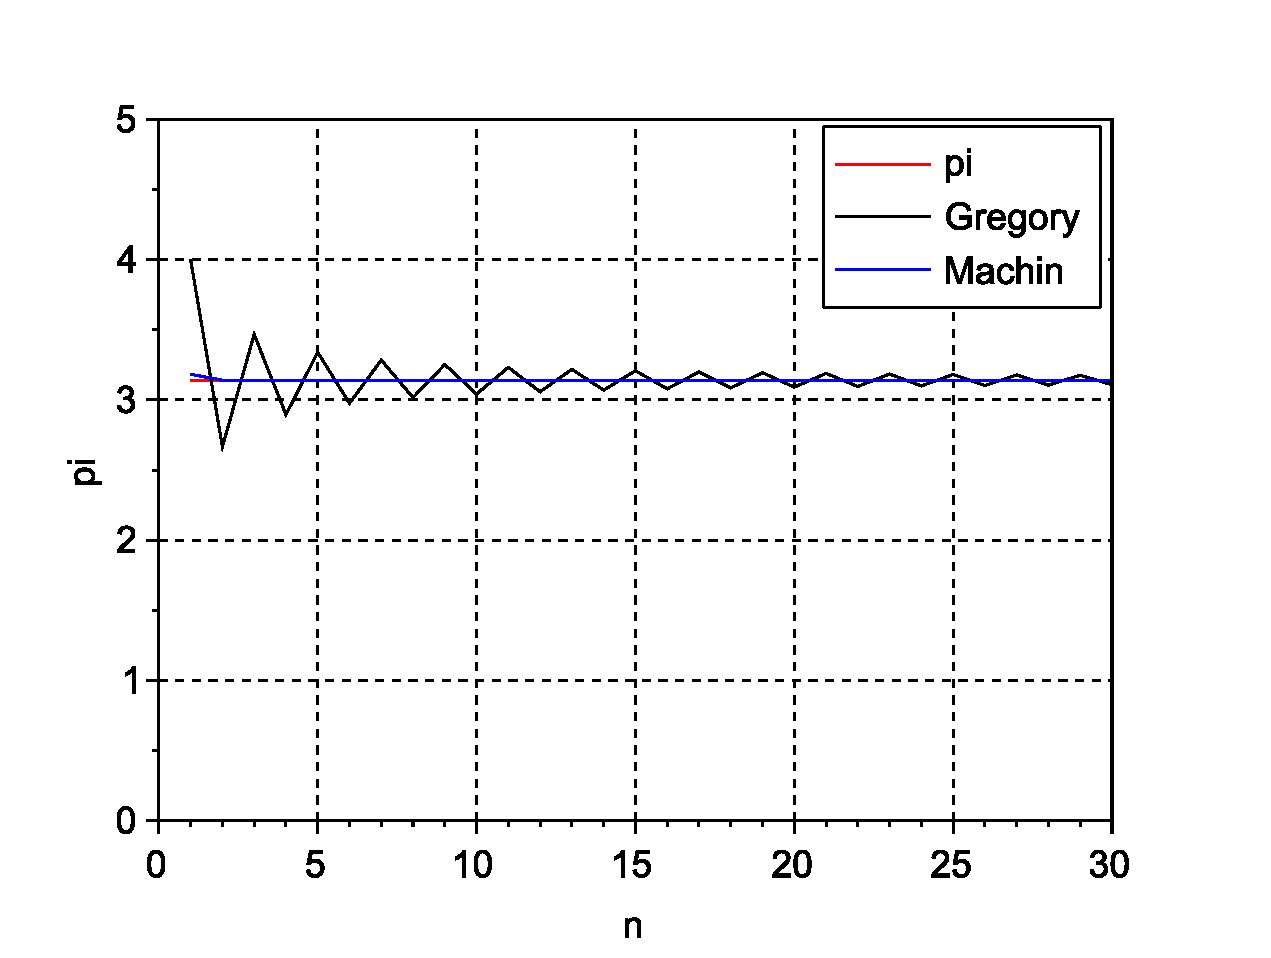
\includegraphics[width=8cm]{図3.pdf} & 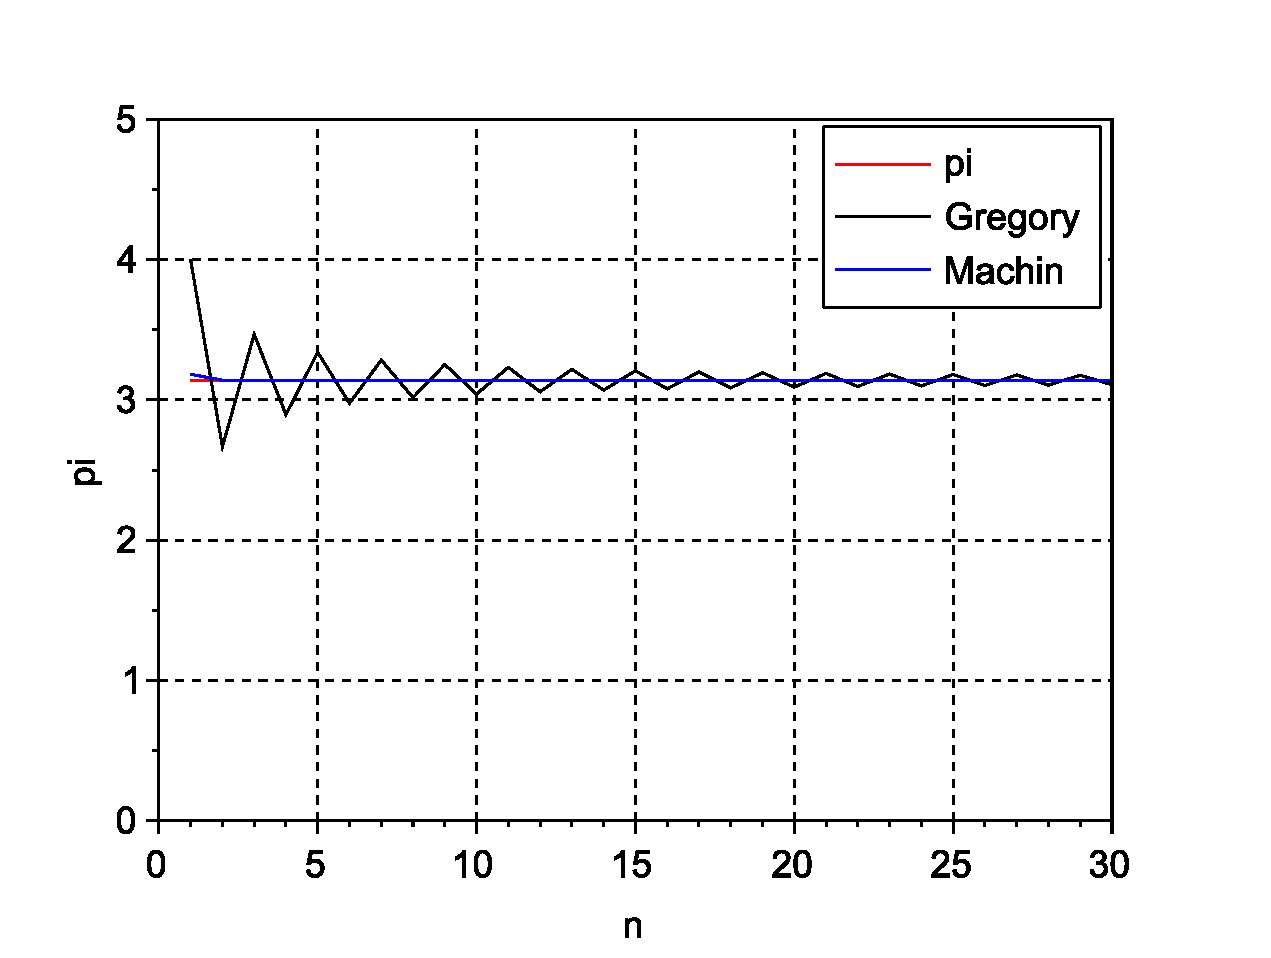
\includegraphics[width=8cm]{図3.pdf} \\
    (a) & (b) \\
    \hline
    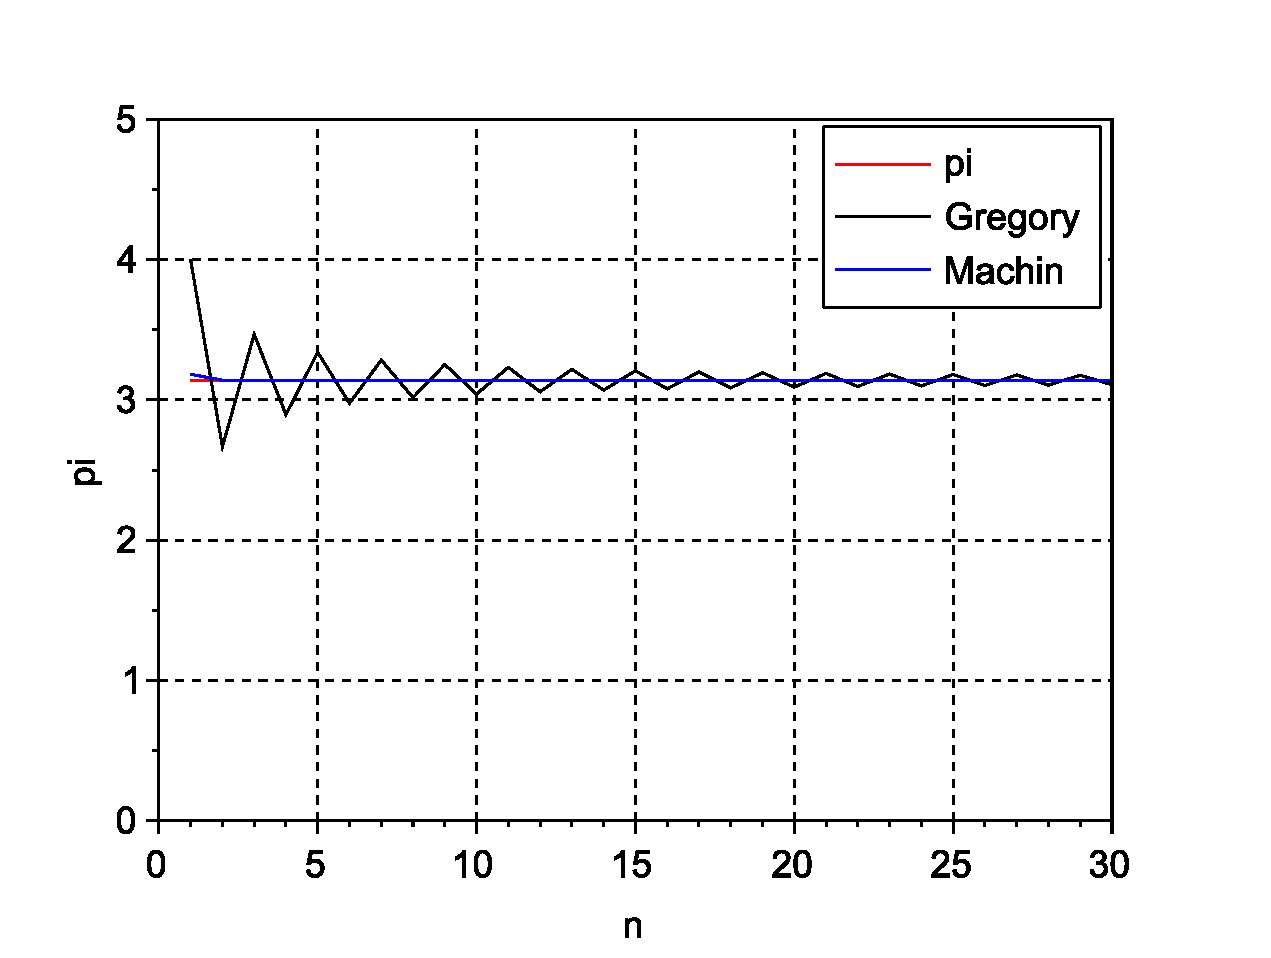
\includegraphics[width=8cm]{図3.pdf} & 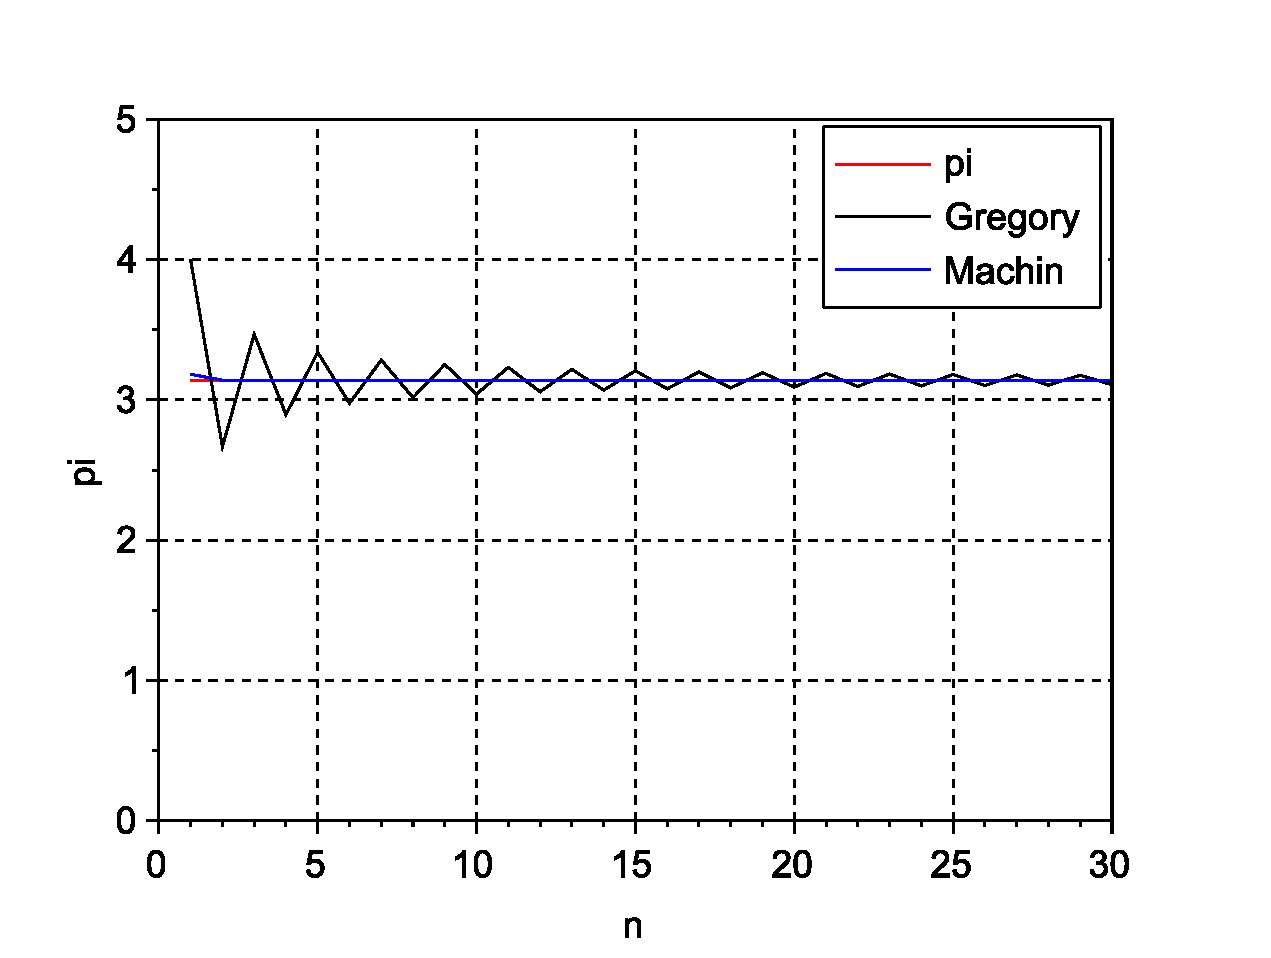
\includegraphics[width=8cm]{図3.pdf} \\
    (c) & (d) \\
    \hline
  \end{tabular}
\end{figure}


%#######################################################################################
\chapter{本論} % <- 本論のタイトルは自分の内容にあったものを考える
%#######################################################################################
数学講究研究報告で述べたい主要な事項（中心的な事項）についてまとめる．
長くなる場合は，3.1，3.2，$\ldots$のように，内容ごとに節に分けてもよい．







%#######################################################################################
\chapter{まとめ}
%#######################################################################################
この研究報告で何について述べ，どのような結果が得られたのかを1ページ程度で簡潔にまとめる．
課題が残った場合は，今後の課題としてそのことを書く場合がある．




%#######################################################################################
\chapter*{付録A　プログラム} 
\addcontentsline{toc}{chapter}{付録A　プログラム}
%#######################################################################################
\lstset{
	%プログラム言語(複数の言語に対応，C,C++も可)
 	language = Python,
 	%背景色と透過度
 	% backgroundcolor={\color[gray]{.90}},
 	%枠外に行った時の自動改行
 	breaklines = true,
 	%自動改行後のインデント量(デフォルトでは20[pt])	
 	breakindent = 10pt,
 	%標準の書体
 	basicstyle = \ttfamily\scriptsize,
 	%コメントの書体
 	commentstyle = {\itshape \color[cmyk]{1,0.4,1,0}},
 	%関数名等の色の設定
 	%classoffset = 0,
 	%キーワード(int, ifなど)の書体
 	%keywordstyle = {\bfseries \color[cmyk]{0,1,0,0}},
 	%表示する文字の書体
 	stringstyle = {\ttfamily \color[rgb]{0,0,1}},
 	%枠 "t"は上に線を記載, "T"は上に二重線を記載
	%他オプション：leftline，topline，bottomline，lines，single，shadowbox
 	frame = tbrl,
 	%frameまでの間隔(行番号とプログラムの間)
 	framesep = 5pt,
 	%行番号の位置
 	numbers = left,
	%行番号の間隔
 	stepnumber = 1,
	%行番号の書体
 	numberstyle = \tiny,
	%タブの大きさ
 	tabsize = 4,
 	%キャプションの場所("tb"ならば上下両方に記載)
 	captionpos = t
}

\begin{lstlisting}
import os
import cv2
import numpy as np
from imutils import contours
import matplotlib.pyplot as plt
import glob
from natsort import natsorted
from keras.models import load_model

\end{lstlisting}



%#######################################################################################
\chapter*{謝辞} \addcontentsline{toc}{chapter}{謝辞}
%#######################################################################################
お世話になった方々への謝辞を書きます．
インターネット上に，いろいろな例文があるので調べてみてください． 




 


%#######################################################################################
\renewcommand{\bibname}{参考文献} \addcontentsline{toc}{chapter}{参考文献}
%#######################################################################################
\begin{thebibliography}{99}
  \bibitem{1} 今野 紀雄，井手 勇介，複雑ネットワーク入門，講談社，2008．
  \bibitem{2} 尾畑 伸明，数理統計学の基礎， 共立出版， 2014．
  \bibitem{3} Albert-L\'aszl\'o Barab\'asi, R\'eka Albert, 
                 Emergence of scaling in random networks, 
                 {\it Science}, \textbf{286}, pp.509--512, 1999. 
\end{thebibliography}

少しでも参考にした論文や専門書を参考文献として最後に記す．
書き方は，本の場合は上記の\cite{1,2}を，論文の場合は上記の\cite{3}を参考にしてください．
また，本文中のどこで参考にしたかを，「先行研究では，...という結果が得られている\cite{3}．」のように，参考にした箇所で適切に示すとよい． 

教科書でわからないことがあった場合は，教科書の参考文献から調べていくと，目的の情報が見つかりやすい．
図書館，図書館の書庫，インターネットで論文名を検索するなど，いろいろな方法で調べてみるとよい．

\end{document}
%%%%%%%%%%%%%%%%%%%%%%%%%%%%%%%%%%%%%%%%%%%%%%%%%%%%%%%%%%%%%%%%%%%%%%%%%%%%%%%%%%%%%%%%